\documentclass[12pt,a4paper]{cv}

\begin{document}

%--------------------------------------------------
% HEADING
%--------------------------------------------------
\parbox{25mm}{%
	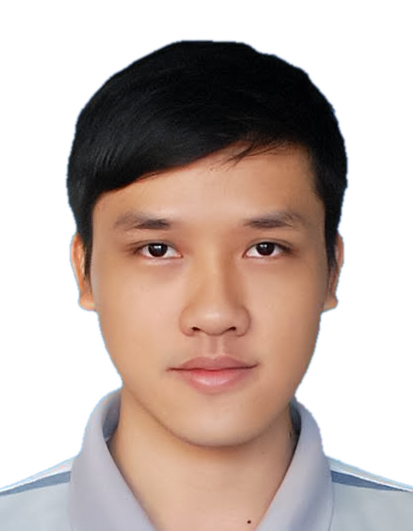
\includegraphics[width=2.35cm,clip]{avt.jpg}
}
\parbox{\dimexpr\linewidth-25mm}{
	\begin{tabularx}{\linewidth}{X r}
		\cvName{Thinh}{Nguyen Phuoc} & \\
		\textit{Software Engineer} & (+84)989 098 494 \\
		& September 26, 1996 \\
		& \href{mailto:npthinh1996@gmail.com}{npthinh1996@gmail.com} \\
		Tan Binh District & \href{https://www.linkedin.com/in/thinh9e/}{linkedin.com/in/thinh9e} \\
		Ho Chi Minh City, VN & \href{https://thinhblog.com}{thinhblog.com}
	\end{tabularx}
}
\medskip
\\
Software Engineer with over 5 years of experience developing high-performing Python and Java applications in Agile environments. Demonstrated expertise in optimizing database queries, enhancing security, and collaborating with teams to deliver impactful results.
\bigskip


%--------------------------------------------------
% EDUCATION
%--------------------------------------------------
\begin{cvSection}{Education}

	\textbf{Ho Chi Minh City University of Technology} \hfill \textit{Sep 2014 -- Nov 2019} \\
	B.S. in Computer Science \& Engineering \\
	Overall GPA: 7.42

\end{cvSection}


%--------------------------------------------------
% WORK EXPERIENCE
%--------------------------------------------------
\begin{cvSection}{Work Experience}

	\begin{cvSubsection}{TMA Solutions}{Mar 2019 -- Present}{Software Engineer}
		\item Contributed to a network performance monitoring project.
		\item Resolved critical customer issues, including system hangs, database errors, and installation problems.
		\item Optimized query execution times by strategic indexing and efficient joins, addressing system bottlenecks to enhance application performance.
		\item Collaborated on new feature implementations, improving user experience and system functionality.
		\item Identified and mitigated security vulnerabilities, preventing potential breaches such as SQL injection and XSS.
		\item Developed Python automation tools to streamline tasks, reducing errors and increasing productivity.
	\end{cvSubsection}

%--------------------------------------------------

	\begin{cvSubsection}{MangoAds}{Jun 2018 -- Aug 2018}{Intern}
		\item Automated content collection and import for WordPress pages using plugins.
		\item Created a PHP and Scrapy tool to input keywords and track their rankings on top search engines like Google and Bing.
		\item Pursued courses on Udemy to continuously enhance skills.
	\end{cvSubsection}

\end{cvSection}


%--------------------------------------------------
% SKILL
%--------------------------------------------------
\begin{cvSection}{Skill}

	\begin{tabular}{@{} >{\bfseries}l @{\hspace{6ex}} l @{}}
		Programming Languages & Python, Java, C/C++ \\
		Frameworks & Django, Spring, Hugo, Bootstrap \\
		Databases & MariaDB, SQL Server \\
		Tools & Git, SVN, Docker, Burp Suite \\
		AI & Rasa, LangChain, Ollama
	\end{tabular}

\end{cvSection}


%--------------------------------------------------
% PERSONAL PROJECT
%--------------------------------------------------
\begin{cvSection}{Personal Project}

	\begin{cvSubsection}{Web Checker}{Dec 2018 -- Present}{
			Project URL: \cvLinkURL{https://github.com/thinh9e/web-checker}
		}
		\item Developed a Django-based web application to assess SEO scores using the MVC pattern.
		\item Implemented URL input functionality, content retrieval, XPath parsing, and link status analysis to identify missing items and generate scores.
		\item Utilized ThreadPool for concurrent request handling, significantly reducing response time.
	\end{cvSubsection}

%--------------------------------------------------

	\begin{cvSubsection}{Burp Suite Automation}{Aug 2021 -- Jun 2023}{}
		\item Created a custom tool for web app content crawling with Burp Suite proxy integration.
		\item Used Selenium for web browser automation and Tkinter for an interactive GUI.
		\item Deployed the tool at TMA Solutions to enhance security scanning automation in project workflows.
	\end{cvSubsection}

%--------------------------------------------------

	\begin{cvSubsection}{Checksum Generator}{Dec 2021 -- Dec 2021}{}
		\item Developed a Python-based checksum generation tool for critical files in the installations directory to enhance data integrity.
		\item Implemented JSON configuration loading to track file additions, modifications, and deletions, updating corresponding checksum files.
		\item Integrated the tool with TMA Solutions project, ensuring seamless functionality in the installation binaries delivered to customers.
	\end{cvSubsection}

\end{cvSection}


%--------------------------------------------------
% CERTIFICATE
%--------------------------------------------------
\begin{cvSection}{Certificate}

	\begin{cvSubsection}{Intermediate to Advanced Python with 10 OOP Projects}{Jan 2024}{
			Udemy: \cvLinkURL{https://ude.my/UC-31536a7e-1d52-4cb2-b73d-60bbe5525a33/}
		}
		\item[] Mastered Python with proficiency in OOP, Git, APIs, databases, deployment, PEP8, and more.
	\end{cvSubsection}

%--------------------------------------------------

	\begin{cvSubsection}{Python Django Dev To Deployment}{Nov 2018}{
			Udemy: \cvLinkURL{https://ude.my/UC-PRMHJ580/}
		}
		\item[] Developed and deployed a real estate application using the Django framework and PostgreSQL.
	\end{cvSubsection}

%--------------------------------------------------

	\begin{cvSubsection}{Python and Django Full Stack Web Developer Bootcamp}{Sep 2018}{
			Udemy: \cvLinkURL{https://ude.my/UC-53QB9QRM/}
		}
		\item[] Gained experience in web development with expertise in HTML, CSS, Bootstrap, JavaScript, jQuery, Python 3, and Django.
	\end{cvSubsection}

\end{cvSection}


%--------------------------------------------------
% AWARD
%--------------------------------------------------
\begin{cvSection}{Award}

	\begin{cvSubsection}{AI Contest 2023}{Oct 2023}{TMA Solutions -- DG}
		\item Secured third place in an AI contest.
		\item Developed an AI chatbot that seamlessly integrated with customer systems.
		\item Skilled in creating solutions for answering FAQs and interacting with system services via REST API.
	\end{cvSubsection}

\end{cvSection}

\end{document}
